\chapter{Desenvolvimento}

\section{Escolha do produto e refrigerante}

    Para o início do projeto, decidiu-se que o produto a ser resfriado seria o peixe, transportado e armazenado em temperatura comercial. As propriedades do produto, bem como as temperaturas de operação estão de acordo com \ref{massa peixe}. 

    Com o produto definido, partiu-se para a definição do fluido refrigerante, em virtude do seu baixo custo e disponibilidade, o fluido refrigerante $R-134A$ se mostrou o mais apto para a realização da operação proposta.

\section{Estimativa da taxa de calor necessário de resfriamento}

    Para a escolha do compressor a ser utilizado, primeiramente foi estimado a taxa de calor a ser retirada do sistema, a partir da Equação \ref{Q resfriamento}. Como temos o volume, o tempo de pulldown e o material a ser refigerado, podemos calcular a carga térmica mínima necessária.

\begin{equation}
    m_{peixe} = \rho V_{refrigerador}
    \label{massa peixe}
\end{equation}

\begin{equation}
    \dot{Q} = m c \Delta T / \Delta t
    \label{Q resfriamento}
\end{equation}


\begin{table}[h]
\centering
\begin{tabular}{|c|c|}
\hline
$\rho$ {[}kg/m³{]} & 972 \\ \hline
$V_{refrigerador}$ {[}m³{]}     & 0.14 \\ \hline
$c$ {[}J/kgK{]}     &  1.71 \\ \hline
$\Delta T$ {[}K{]}     &  25 \\ \hline
$\Delta t$ {[}s{]}     &  $2.88 \cdot10^{4}$ \\ \hline
\end{tabular}
\caption{Valores utilizados.}
\label{tab:tabela dados}
\end{table}

Obtemos:
\begin{equation}
    \dot{Q} = 202.6 W
    \label{carga}
\end{equation}

Com a carga térmica definida, é necessário selecionar um compressor adequado para a operação. Para isso, será utilizado o seletor de produtos disponível no site do fabricante Embraco \textcopyright. Para a aplicação em questão, que envolve baixas temperaturas, recomenda-se a utilização de compressores do tipo LBP. Uma vez selecionados os compressores que atendiam aos requisitos, os dados de operação individuais foram obtidos no site do fabricante.

\begin{figure}
    \centering
    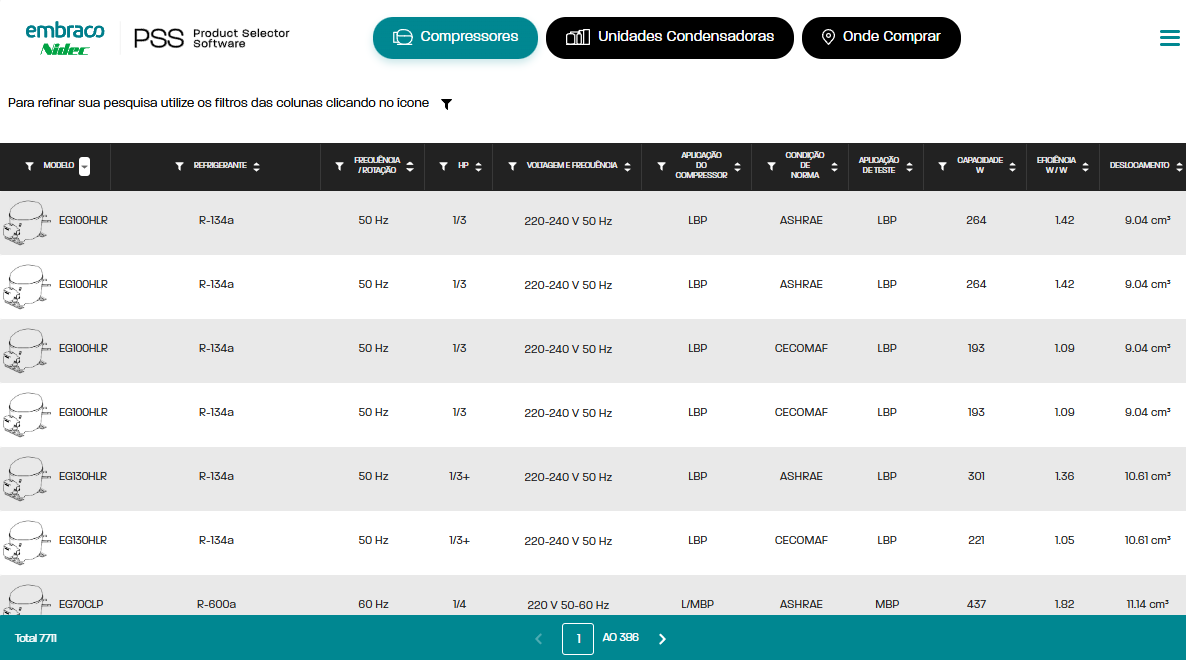
\includegraphics[width=0.8\linewidth]{Imagens/Desenvolvimento/PSS-embraco.png}
    \caption{Seletor de produtos.}
    \label{fig:seletor de produtos}
\end{figure}

\newpage

O documento contém as temperaturas de condensação e evaporação empregadas nos testes de desempenho, além de parâmetros como capacidade de refrigeração, consumo de energia, corrente elétrica, entre outros. Dessa maneina, foram selecionas os compressores descrtitos na Tabela \ref{tab:compressores escolhidos}.


\begin{table}[h]
\centering
\begin{tabular}{|c|c|}
\hline
Modelo    & Potencia {[}W{]} \\ \hline
EGAS80HLR & 240              \\ \hline
EGZS60HLP & 180              \\ \hline
EGZS70HLC & 202              \\ \hline
FFU70HAK  & 221              \\ \hline
\end{tabular}
\caption{Compressores escolhidos.}
\label{tab:compressores escolhidos}
\end{table}

\section{Ciclo de Refrigeração Padrão:}

Com os dados preliminares obtidos, foi desenvolvida uma rotina em Python para calcular as propriedades do sistema, de acordo com o ciclo descrito na Figura \ref{fig:ciclo padrão}. 

\begin{figure}
    \centering
    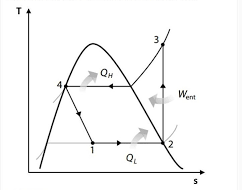
\includegraphics[width=0.6\linewidth]{Imagens/Desenvolvimento/Diagrama.png}
    \caption{Ciclo padrão.}
    \label{fig:ciclo padrão}
\end{figure}

\newpage

O programa utiliza um método iterativo para determinar a  mínima temperatura operacional possível, com o objetivo de reduzir custos ao evitar o superdimensionamento do compressor, utilizando como base os parâmetros descritos a seguir:

\begin{equation}
    \dot{Q_L} = \dot{m}(h_1-h_4)
    \label{QL}
\end{equation}

\begin{equation}
    \dot{Q_H} = \dot{m}(h_2-h_3)
    \label{QH}
\end{equation}

    Onde $\dot{Q_L}$ e $\dot{Q_H}$, são  a taxa com que sai e que entra calor no sistema, respectivamente. O trabalho do compressor pode ser calculado apartir da equação \ref{W compressor}, utilizando as propriedades do fluido antes e depois da compresão.

\begin{equation}
    \dot{W_{comp}} = \dot{m}(h_2-h_1)
    \label{W compressor}
\end{equation}

\begin{equation}
    \Delta h_{1-2} \simeq  c_p (T_2-T_1)
    \label{simplificacao entalpia}
\end{equation}

    E a eficiência do sistema é dada como:

\begin{equation}
    COP = \frac{T_H}{T_H - T_L}
    \label{COP carnot}
\end{equation}

\newpage    

Simultaneamente, são calculadas as propriedades do fluido refrigerante em cada estado do ciclo de refrigeração. Para efeito de comparação com o ciclo real, também é realizado o cálculo do ciclo ideal de Carnot, a fim de se obter a eficiência máxima possível e as temperaturas mínimas requeridas pelo sistema.

Depois de uma rodada de anállises, dois compressores destacaram-se, o desempenho de ambos nos ciclos pode ser visto nas figuras \ref{fig:ciclo comp 1} e \ref{fig:ciclo comp 2}.

\begin{figure}[h]
    \centering
    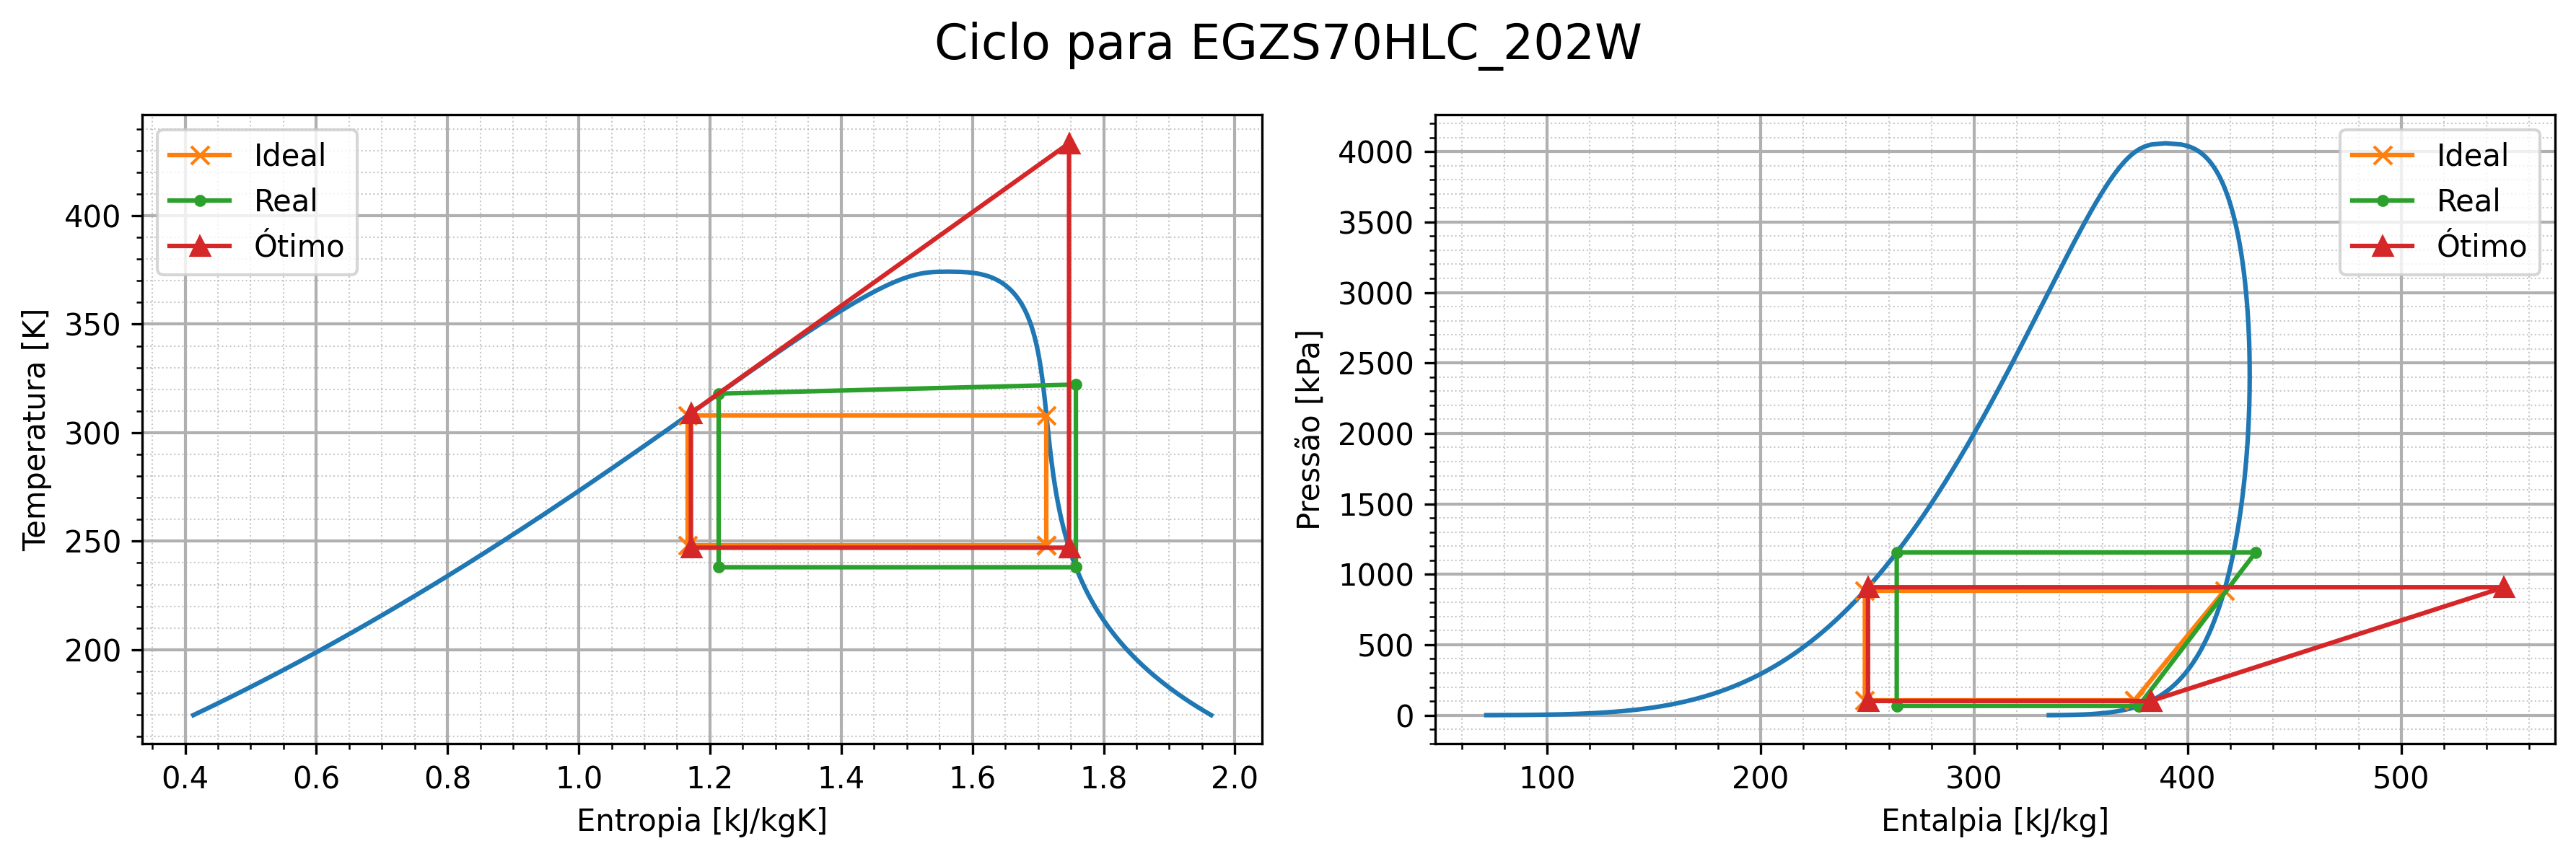
\includegraphics[width=0.9\linewidth]{Imagens/Desenvolvimento/ciclo_EGZS70HLC_202W.png}
    \caption{Ciclo para o EGZS70HLC.}
    \label{fig:ciclo comp 1}
\end{figure}

\begin{figure}[h]
    \centering
    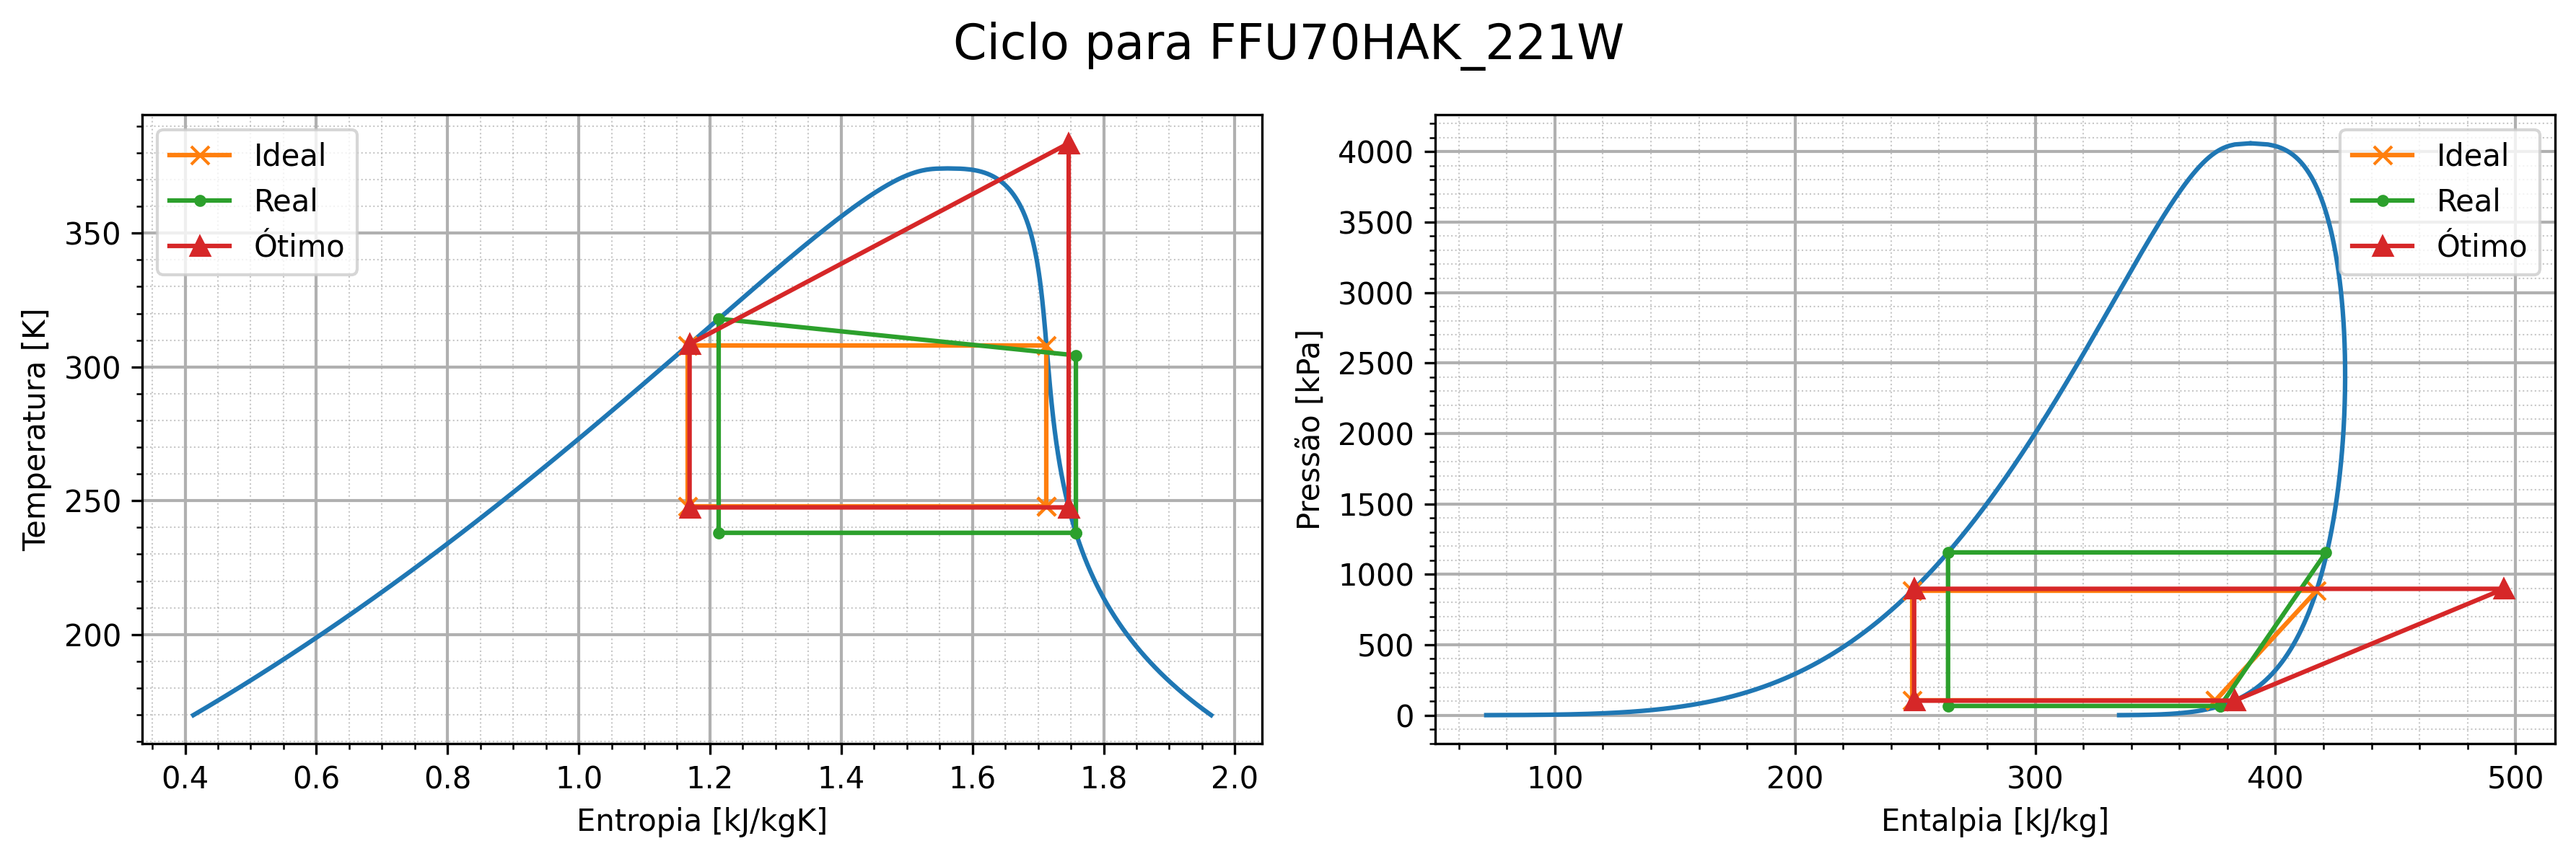
\includegraphics[width=0.9\linewidth]{Imagens/Desenvolvimento/ciclo_FFU70HAK_221W.png}
    \caption{Ciclo para o FFU70HAK.}
    \label{fig:ciclo comp 2}
\end{figure}

É possivél notar uma grande diferença entre o ciclo real e o ótimo, causada pelas perdar do sistema real, que aparecem em forma de calor. A rotina desenvolvida também calcula outros parâmetros de desempenho do sistema, tais como fluxo mássico, potência, COP e ${Q_L}$.

\newpage

\begin{figure}[h]
    \centering
    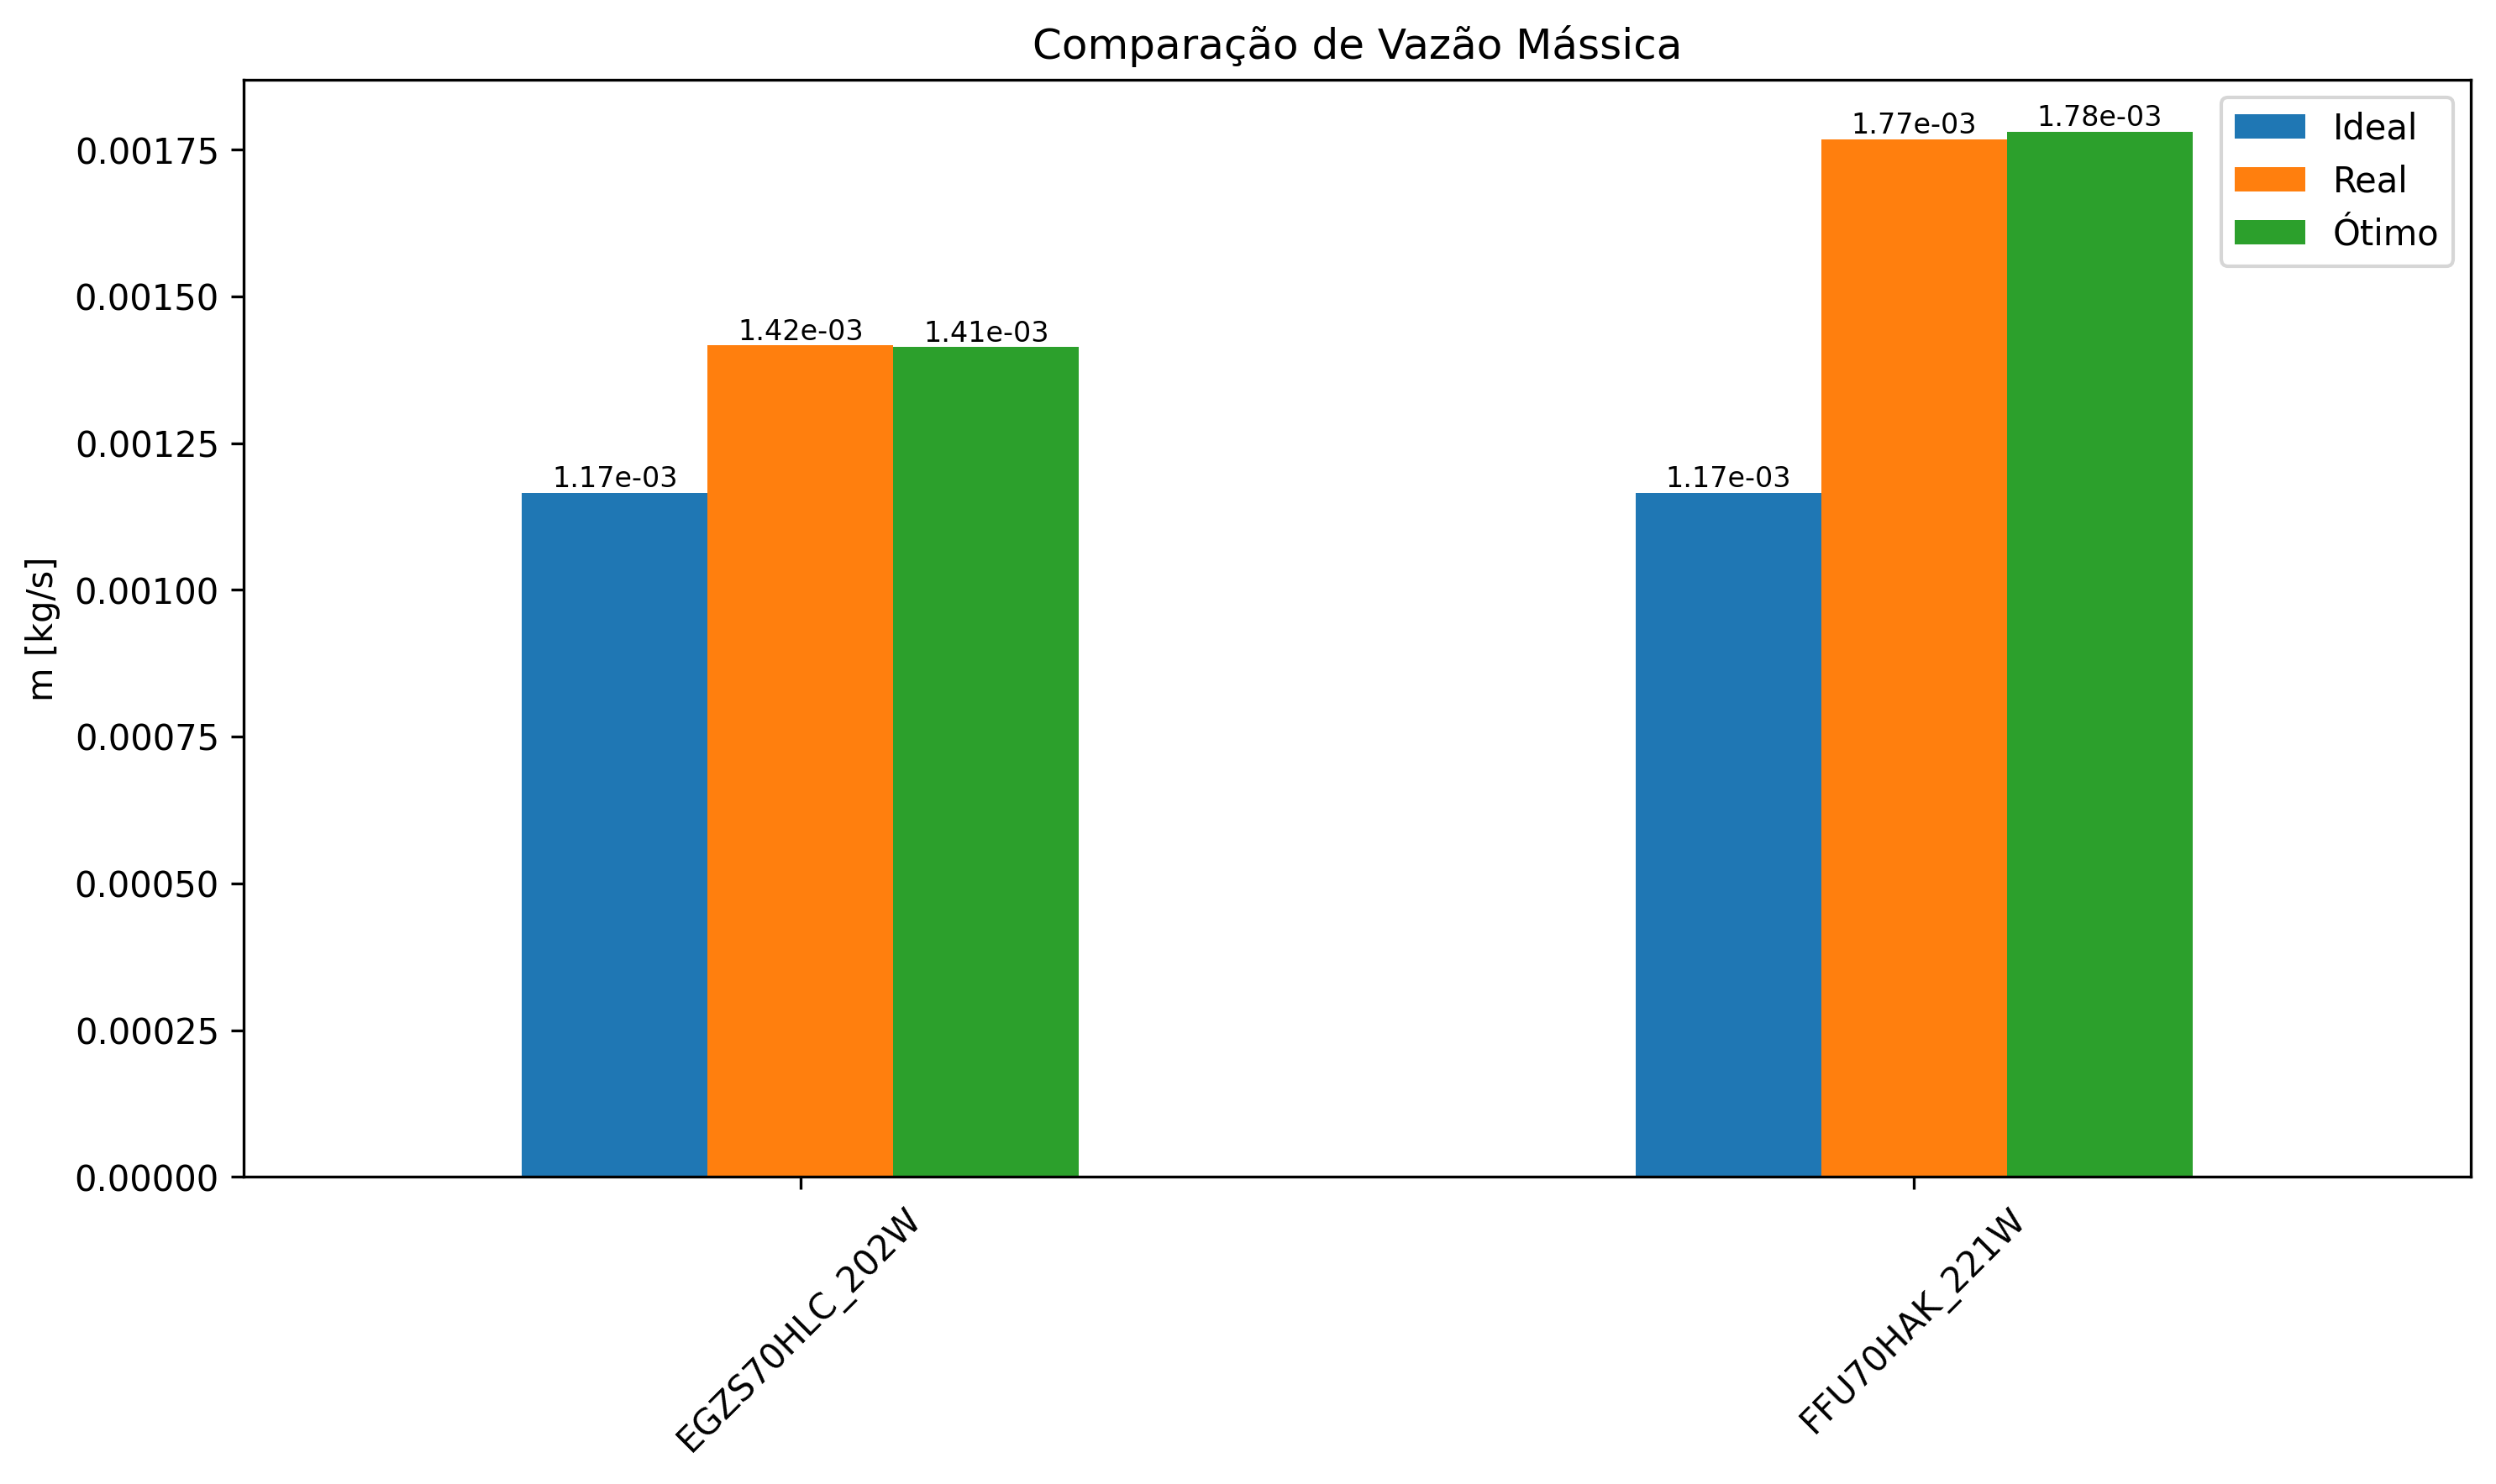
\includegraphics[width=0.8\linewidth]{Imagens/Desenvolvimento/barras_m.png}
    \caption{Compração do $\dot{m}$.}
    \label{fig:barras fluxo massa}
\end{figure}

\begin{figure}[h]
    \centering
    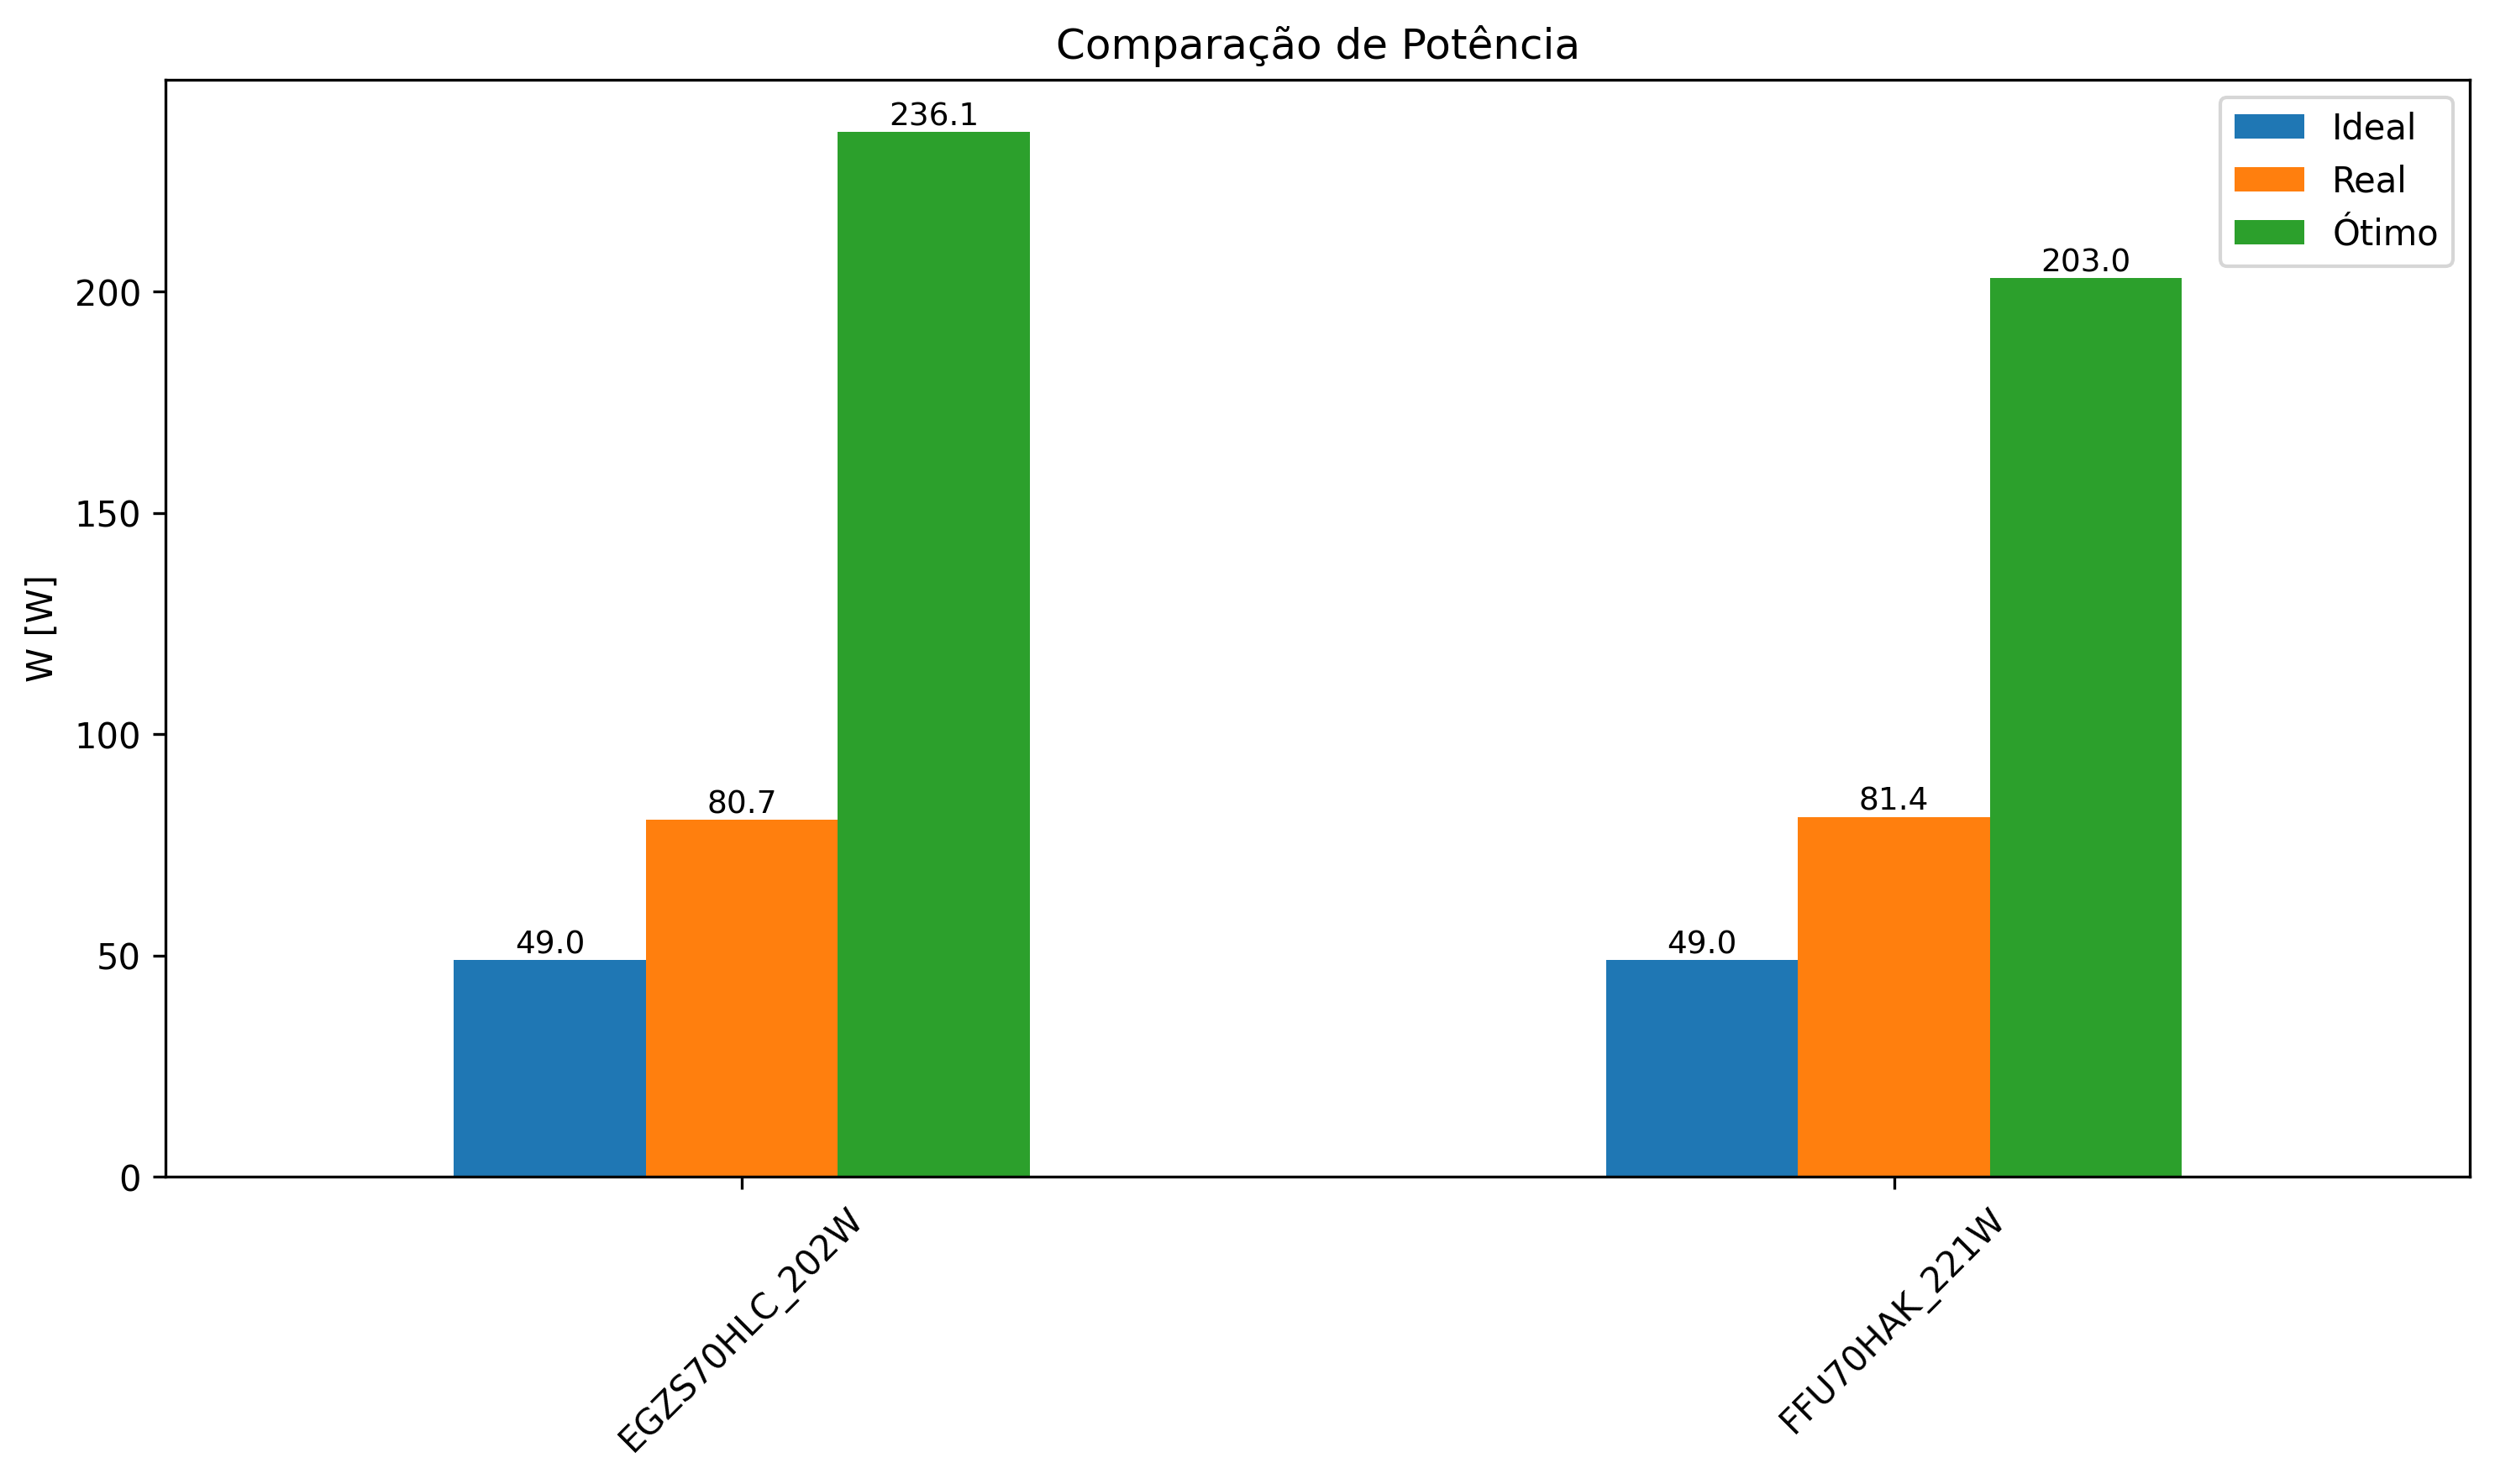
\includegraphics[width=0.8\linewidth]{Imagens/Desenvolvimento/barras_W.png}
    \caption{Compração da potência.}
    \label{fig:barras W}
\end{figure}

\newpage

\begin{figure}[h]
    \centering
    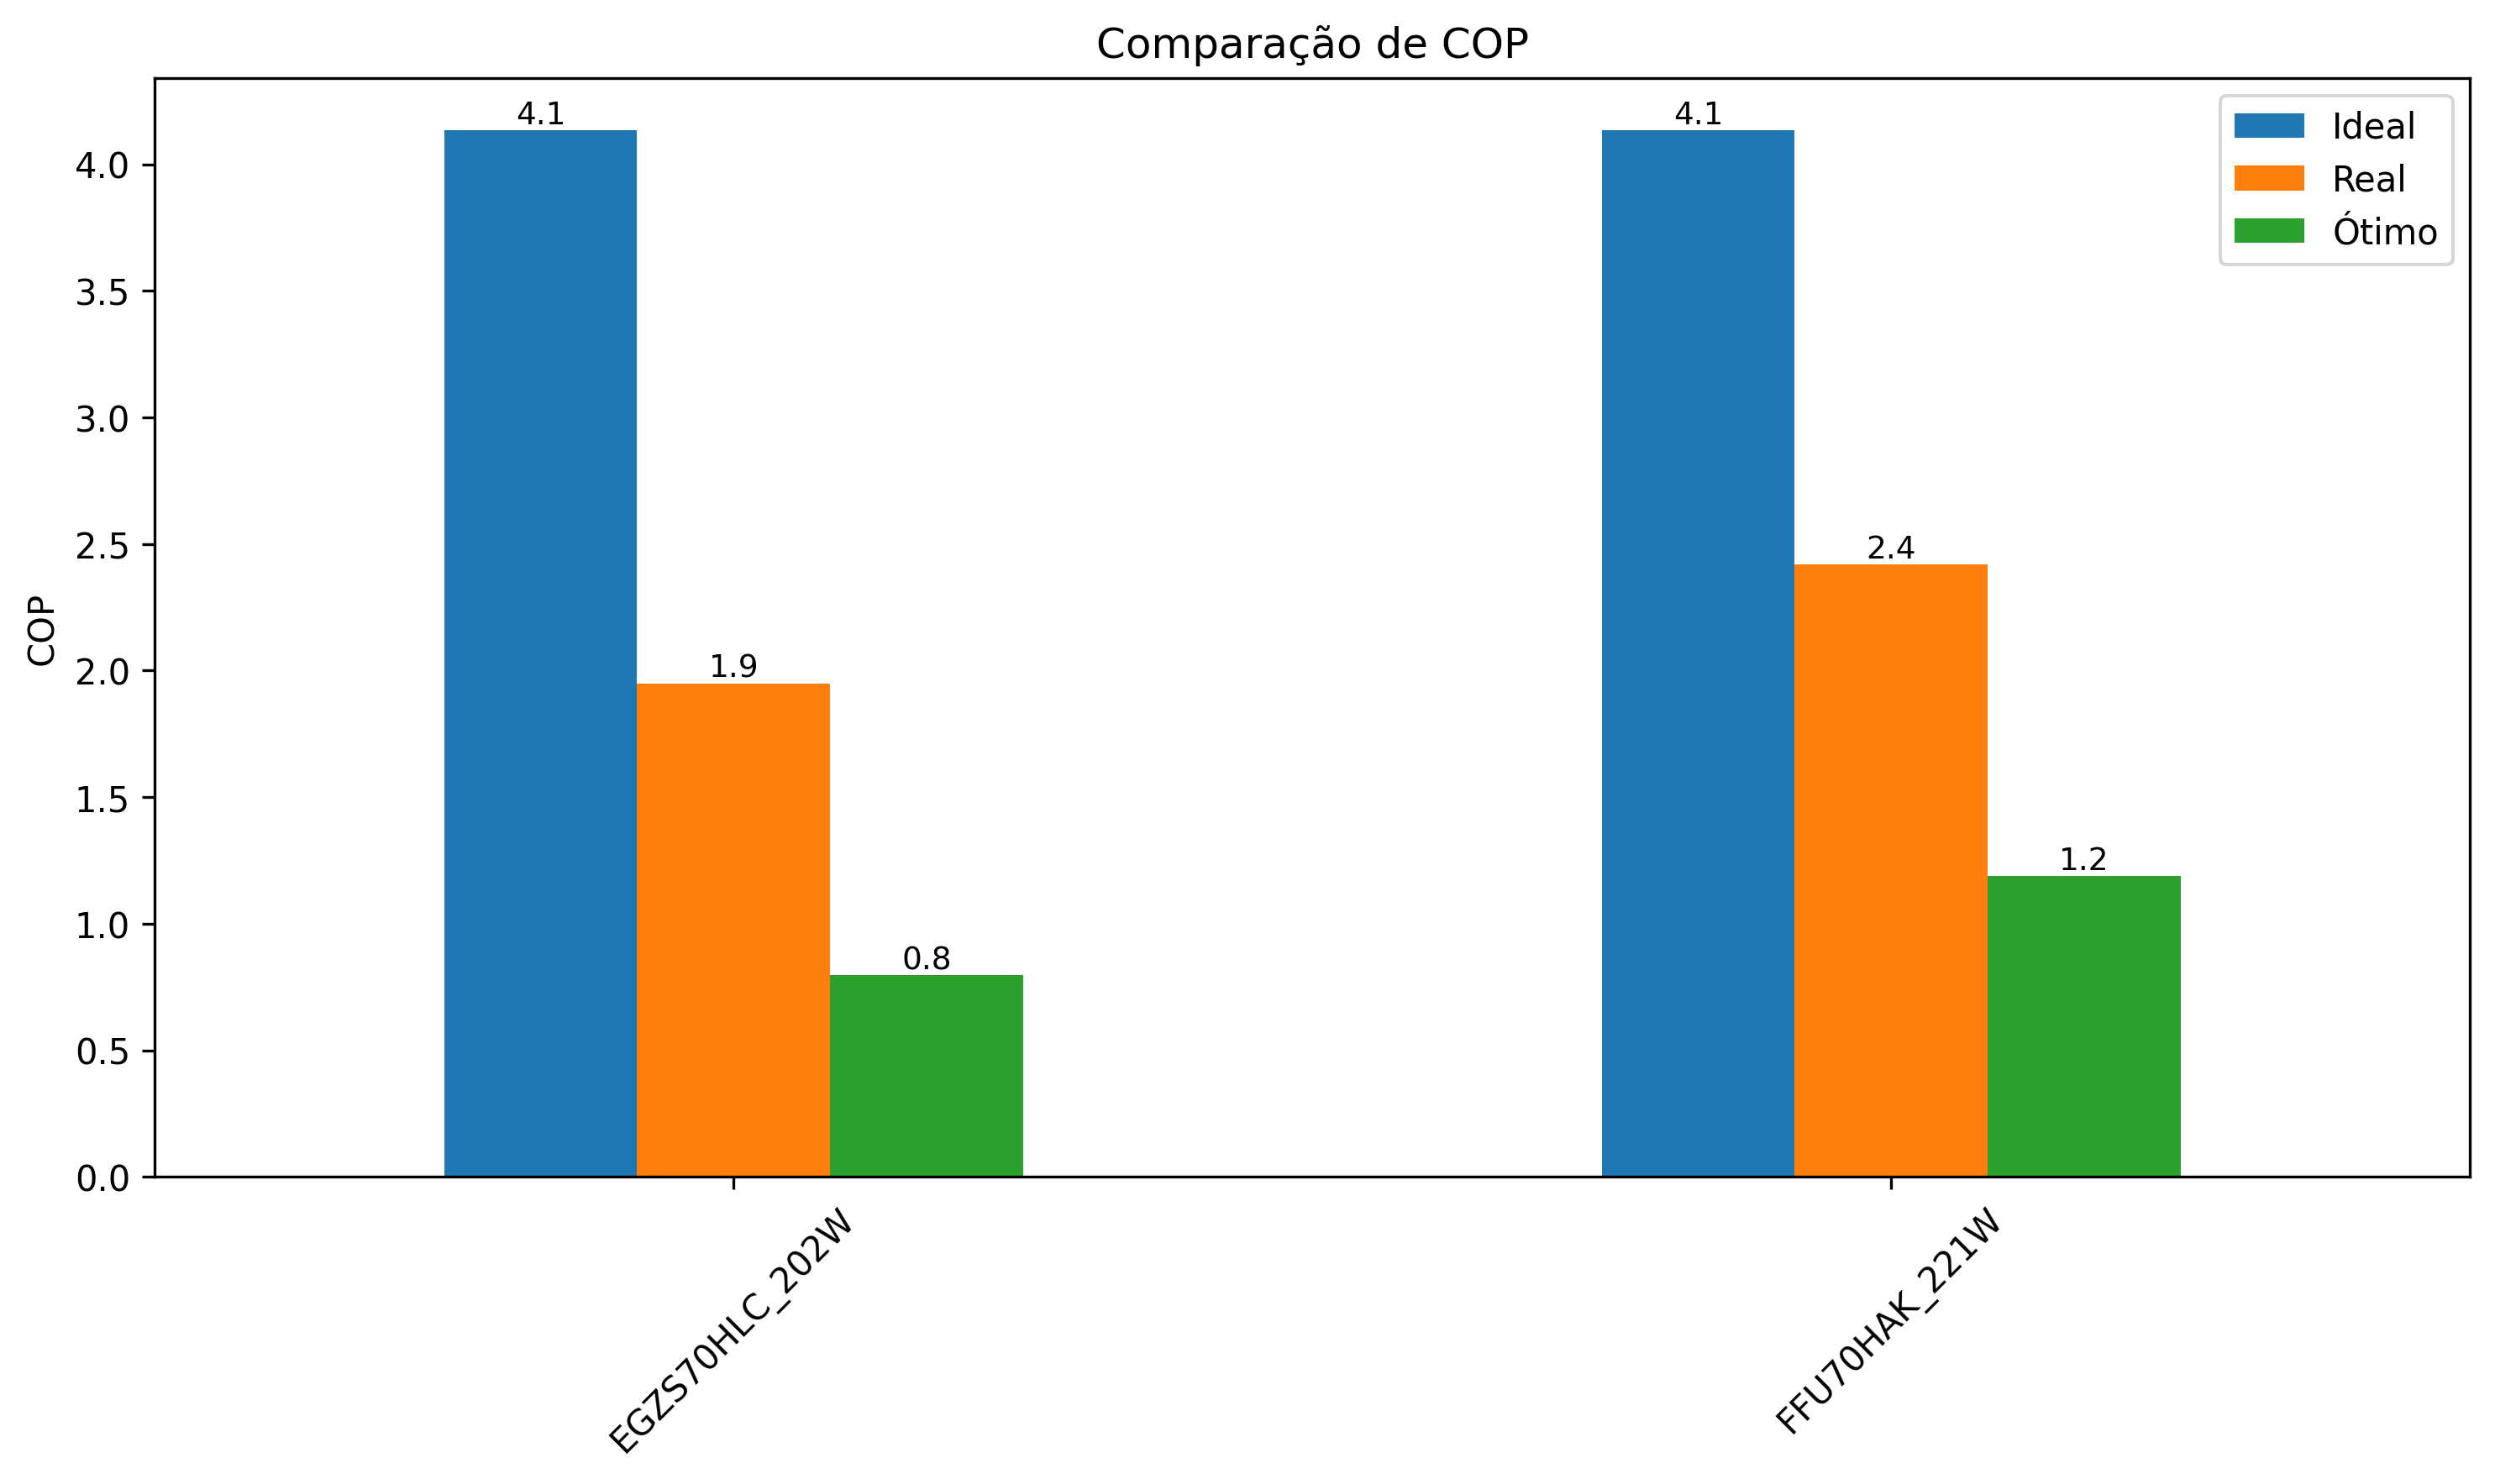
\includegraphics[width=0.8\linewidth]{Imagens/Desenvolvimento/barras_COP.png}
    \caption{Compração do COP.}
    \label{fig:barras COP}
\end{figure}

\begin{figure}[h]
    \centering
    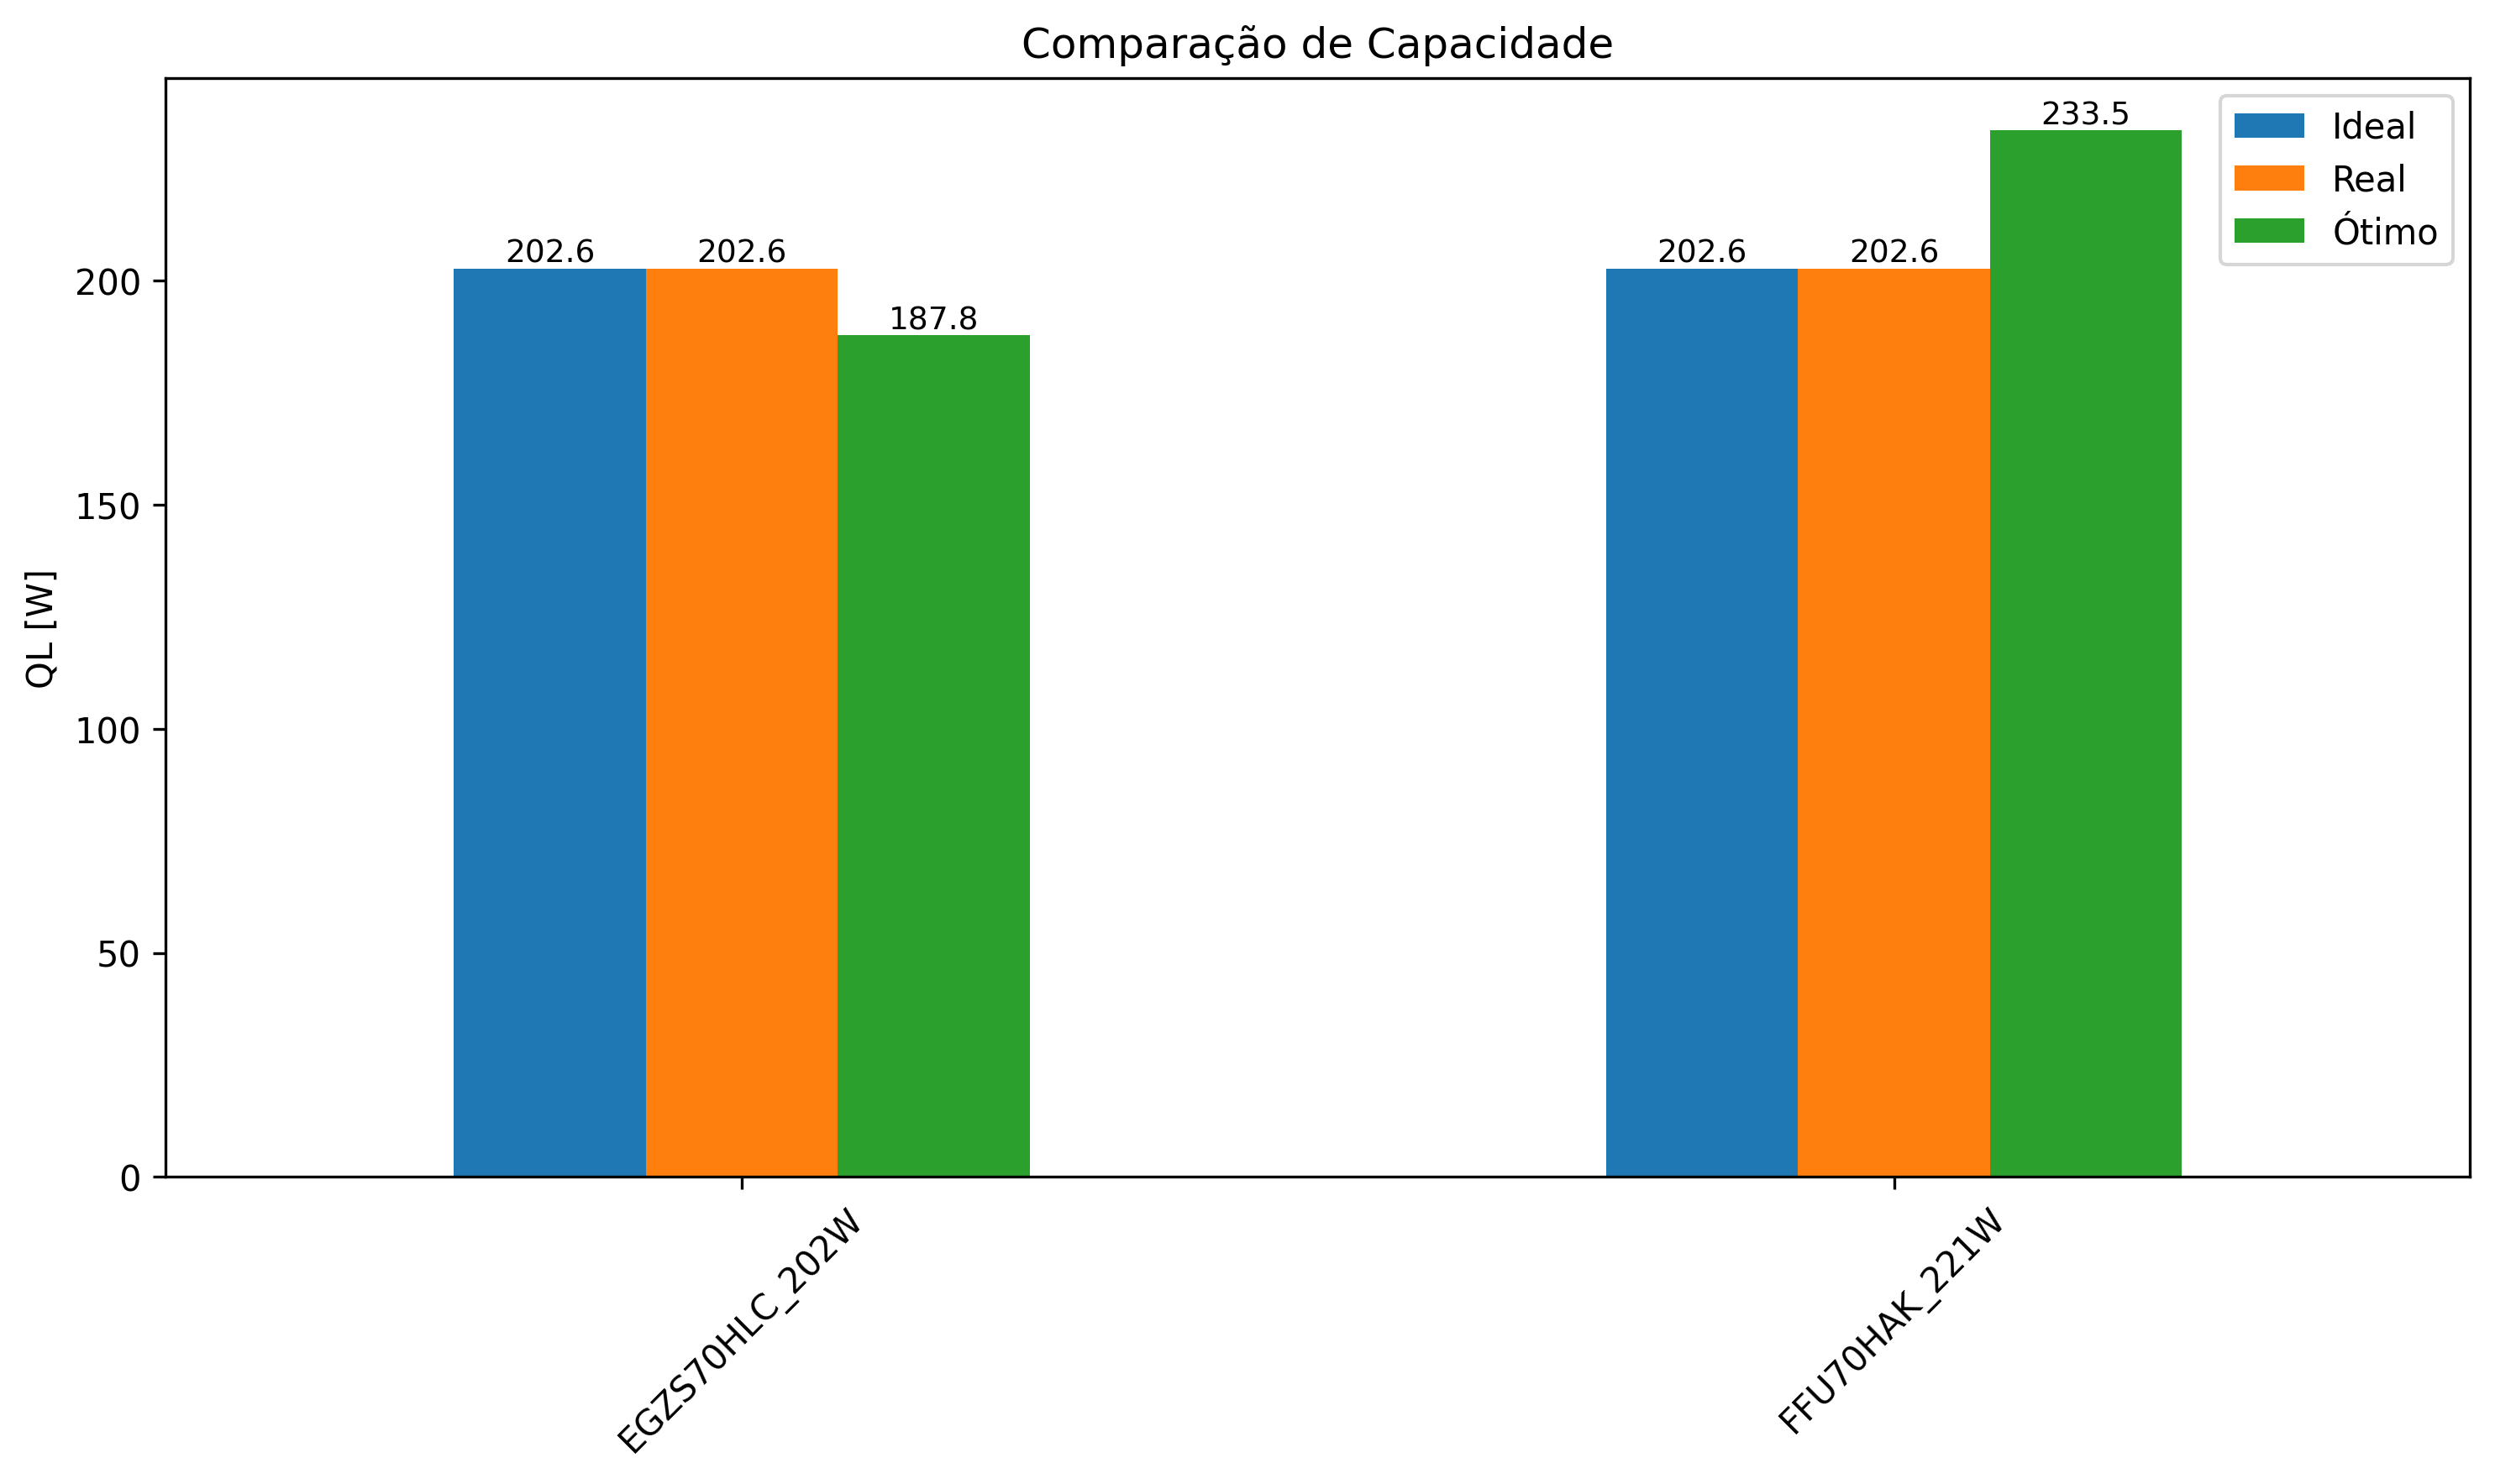
\includegraphics[width=0.8\linewidth]{Imagens/Desenvolvimento/barras_QL.png}
    \caption{Compração do $Q_L$.}
    \label{fig:barras Ql}
\end{figure}



Os resultados obtidos e mostrados nas Figuras \ref{fig:barras fluxo massa} a \ref{fig:barras Ql} demonstram a fidelidade do modelo computacional calculado com a base teórica, com  cada propriedade apresentando um comportamento esperado em cada situação.

    \begin{itemize}
        \item $\dot{m}$ : O ciclo ideal apresentou o menor valor para o fluxo mássico, enquanto os ciclos reais e ótimos aparecem com valores ligeiramente maiores, isso acontece pela necessidade de uma maior retirada de calor no sistema.
        \item COP : A máxima eficiência possível é determinada pelo ciclo de Carnot de refrigeração. A discrepância entre esse valor teórico e o desempenho no sistema real indica o quanto ele se afasta do ideal.
    \end{itemize}

% ver custo dos compressores e ver qual é melhor